\documentclass[default]{beamer}
\setbeamertemplate{navigation symbols}{}

\usetheme{CambridgeUS}
\useoutertheme{infolines}
%\usecolortheme{crane}

\usepackage{cmap}	% Поддержка поиска русских слов в PDF (pdflatex)
\usepackage[T2A]{fontenc}       %поддержка кириллицы
\usepackage[utf8]{inputenc}	% Выбор языка и кодировки
\usepackage[english, russian]{babel}
%\usepackage[unicode]{hyperref}			% Русский язык для оглавления pdf
\usepackage{bookmark}					% Оглавление в pdf

\usepackage{color}
\usepackage{listings}

\graphicspath{{../../images/oop/}} 			% Пути к изображениям

\makeatletter
\setbeamertemplate{footline}
{
	\leavevmode%
	\hbox{%
		\begin{beamercolorbox}[wd=.333333\paperwidth,ht=2.25ex,dp=1ex,center]{author
				in head/foot}%
			\usebeamerfont{author in
				head/foot}\insertshortauthor~~\beamer@ifempty{\insertshortinstitute}{}{(\insertshortinstitute)}
		\end{beamercolorbox}%
		\begin{beamercolorbox}[wd=.333333\paperwidth,ht=2.25ex,dp=1ex,center]{title in
				head/foot}%
			\usebeamerfont{title in head/foot}\insertshorttitle
		\end{beamercolorbox}%
		\begin{beamercolorbox}[wd=.333333\paperwidth,ht=2.25ex,dp=1ex,right]{date in
				head/foot}%
			\usebeamerfont{date in head/foot}\insertshortdate{}\hspace*{2em}
			\insertframenumber{}\hspace*{2ex} 
		\end{beamercolorbox}
	}%
	\vskip0pt%
}

\definecolor{mygreen}{rgb}{0,0.6,0}
\definecolor{mygray}{rgb}{0.9,0.9,0.9}
\definecolor{mymauve}{rgb}{0.58,0,0.82}
\lstset{
	backgroundcolor=\color{white},   % choose the background color
	basicstyle=\footnotesize,        % size of fonts used for the code
	breakatwhitespace=true,			 % sets if automatic breaks should only happen at whitespace
	breaklines=true,                 % automatic line breaking only at whitespace
	commentstyle=\color{mygreen},    % comment style
	escapeinside={\%*}{*)},          % if you want to add LaTeX within your code
	keepspaces=true,                 % keeps spaces in text, useful for keeping indentation of code (possibly needs columns=flexible)
	keywordstyle=\color{blue},       % keyword style
	stringstyle=\color{mymauve},     % string literal style
	showspaces=false,                % show spaces everywhere adding particular underscores; it overrides 'showstringspaces'
	showstringspaces=false,          % underline spaces within strings only
	showtabs=false,					 % show tabs within strings adding particular underscores
	tabsize=4,                       % sets default tabsize to 2 spaces
}

\setbeamertemplate{bibliography entry title}{}
\setbeamertemplate{bibliography entry location}{}
\setbeamertemplate{bibliography entry note}{}

\begin{document}
	
	\title[ООП. Лабораторные]{Основы объектно"--~ориентированного программирования.
		Лабораторные}
	\author[Панов]{Александр Панов}
	\institute[МФТИ]{Московский физико-технический институт}
	\date{февраль 2015 г.} 
	
	\begin{frame}
		\titlepage
	\end{frame}
	
	\section {Семинар 1}
	
	\begin{frame}
		\frametitle{Цели курса}
		
		\begin{itemize}
			\item Освоить идеологию объектно"--~ориентированного программирования.
			\item Понять принципы программирования структур данных и типовых решений
			(patterns).
			\item Научиться писать программы на объектно"--~ориентированном языке (Java,
			C++, Python).
			\item Начать создавать безопасные и легко понимаемые программы.
			\item Научиться работать в команде с использованием средств командной
			разработки кода.
			\item Освоить основы параллельного программирования.
			\item Начать пользоваться стандартными и сторонними библиотеками для решения
			своих задачах.
			\item Овладеть инструментами компиляции, отладки и сборки сложных программ.
		\end{itemize}
	\end{frame}
	
	\begin{frame}
		\frametitle{Работа в семестре}
		
		\begin{itemize}
			\item Сформировать команды минимум по 3 человека, максимум "--- 5 (конец
			февраля).
			\item Определиться с языком программирования в команде и темой курсового
			проекта (конец февраля).
			\item Подготовить презентацию своего проекта (конец марта).
			\item Выполнить две семестровых задачи (конец марта).
			\item Сдать курсовой проект (май).
		\end{itemize}
		
		\par\bigskip
		Среда разработки и система контроля версий "--- по своему усмотрению.
	\end{frame}
	
	\begin{frame}
		\frametitle{Литература}
		
		\bibliographystyle{ugost2008}
		\nocite{*}
		\bibliography{../../biblio/misc}
	\end{frame}
			
	\begin{frame}
		\frametitle{TIOBE Index}
		
		Индекс, оценивающий популярность языков программирования. Основан на подсчёте
		результатов поисковых запросов, содержащих название языка (Google, Blogger,
		Wikipedia, YouTube, Baidu, Yahoo!, Bing, Amazon).
		http://www.tiobe.com/index.php/content/paperinfo/tpci/index.html
		
		\begin{columns}
			\begin{column}{0.5\textwidth}
				\begin{figure}
					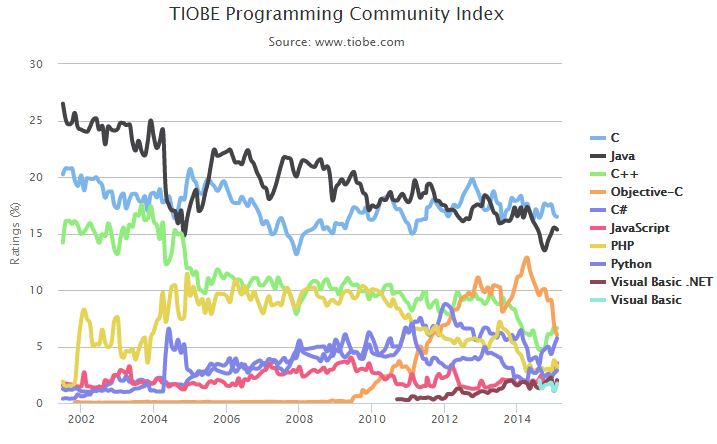
\includegraphics[width=0.8\textwidth]{tiobe_graph}
				\end{figure}
			\end{column}
			\begin{column}{0.5\textwidth}
				\begin{figure}
					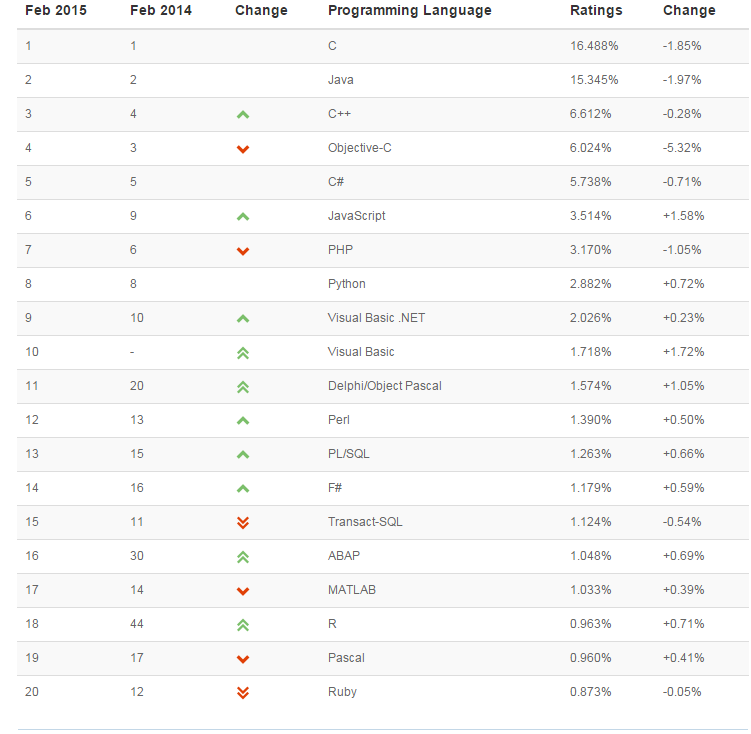
\includegraphics[width=0.8\textwidth]{tiobe_table}
				\end{figure}
			\end{column}	
		\end{columns}
	\end{frame}
	
	\begin{frame}
		\frametitle{ООП на примере языка C++}
		
		\begin{itemize}
			\item История с 1980~г.: изначально <<C with classes>>, крайняя версия "---
			C++11.
			\item Стандартизация с 1996~г. 
			\item Ключевая особенность "--- полная совместимость с C.
			\item Высокая производительность.
			\item Наличие совместимости с C приводит к путанице при использовании
			устаревших функций.
			\item Большое количество библиотек, в том числе и с дублирующими функциями.
		\end{itemize}		
	
	\end{frame}
	
	\begin{frame}
		\frametitle{ООП на примере языка Java}
		
		\begin{itemize}
			\item История с 1995~г.: 6 версий "--- крайняя JDK 1.8.
			\item Поддержка Sun"--~Oracle http://docs.oracle.com/javase/8/docs/
			\item Ключевая особенность "--- программы транслируются в байт-код,
			выполняемый виртуальной машиной Java (JVM). JVM реализована для всех типов
			операционных систем.
			\item Облегченное управление памятью "--- сборка мусора garbage collector
			(GC).
			\item Программные стеки: JavaSE (desktop"--~приложения), JavaEE
			(web"--~приложения), JavaFX (rich"--~приложения), Android (мобильные
			приложения).
			\item Богатый набор уже написанного кода и большое количество библиотек и
			фреймворков (frameworks), решающих огромное количество задач.
		\end{itemize}
	\end{frame}
	
	\begin{frame}
		\frametitle{Компоненты языка Java}
		
		\begin{figure}
			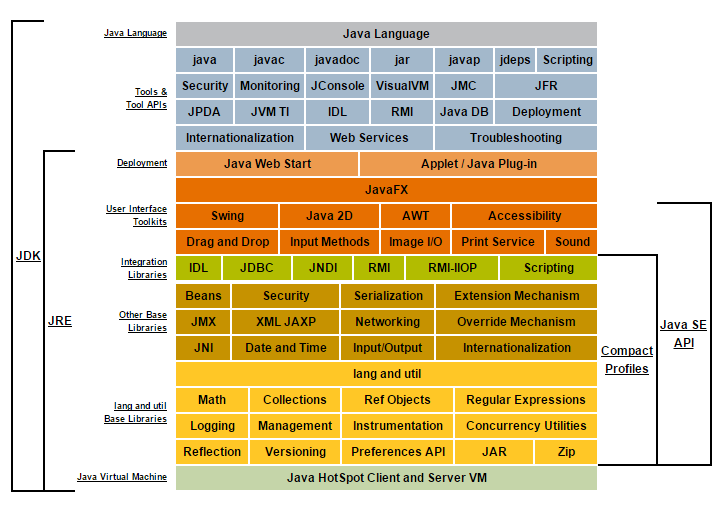
\includegraphics[width=0.8\textwidth]{java_stack}
		\end{figure}
	\end{frame}	
	
	\begin{frame}
		\frametitle{Инструменты языка C++}
		
		\begin{itemize}
			\item STandart Library (STL) "--- библиотека шаблонов.
			\item Boost "--- одна из самых известных библиотек инструментов.
			\item make "--- инструмент сборки программ.
			\item gdb "--- инструмент отладки.
		\end{itemize}
	\end{frame}	

\defverbatim[colored]\lstA{%
\begin{lstlisting}[language=java]
double a = 1, b = 1, c = 6; 
double D = b * b - 4 * a * c; 
if (D >= 0) { 
	double x1 = (-b + Math.sqrt (D)) / (2 * a);
	double x2 = (-b - Math.sqrt (D)) / (2 * a); 
}

int x = 2; 
int y = 0; 
/* if (x > 0) 
		y = y + x*2; 
	else 
		y = -y - x*4; */ 
y = y*y;// + 2*x;
\end{lstlisting}
}
	\begin{frame}
		\frametitle{Примеры на Java}
		
		\lstA
	\end{frame}
	
\defverbatim[colored]\lstB{%
\begin{lstlisting}[language=java]
public class Demo { 

	public static void main (String args[]) {
		System.out.println("Hello, world!");
	}
}
\end{lstlisting}
}

	\begin{frame}
		\frametitle{Hello World! на Java}
		\lstB
		
		\par\bigskip
		Команда компиляции "--- javac Demo.java
		
		Команда запуска скомпилированного приложения "--- java Demo
	\end{frame}
	
	\begin{frame}
	\frametitle{Лексика языка}
	
	\begin{itemize}
		\item Идентификаторы "--- это имена,~которые даются различным элементам языка
		для упрощения доступа к ним. Имена имеют пакеты, классы, интерфейсы, поля,
		методы, аргументы и локальные переменные.
		\item Ключевые слова "--- это зарезервированные слова, состояшие из
		ASCII"--~символов и выполняющие различные задачи языка: abstract, double, int,
		class, public, void и т.~п.
		\item Литералы позволяют задать в программе значения для числовых, символьных и строковых выражений, а также null"--~литералов.
		\item Операторы используются в различных операциях "--- арифмтеических, логических, битовых, опреациях сравнения и присваивания: =, ==, >, <, +, - и т.~п.
	\end{itemize}
	\end{frame}


\defverbatim[colored]\lstC{%
\begin{lstlisting}[language=bash]
ping 64.0.0.0 -c 2 -w2 || wget -qO - "login.telecom.mipt.ru/bin/login.cgi?login=LOGIN &memorize=on&password=
$((wget login.telecom.mipt.ru/bin/getqc.cgi -qO -; echo -n PASSWORD) | md5sum - | head -c32)"
\end{lstlisting}
}	
	\begin{frame}
		\frametitle{Интернет на виртуальных контейнерах}
		\lstC
	
	\end{frame}

	\section{Семинар 2}
	\begin{frame}
		\frametitle{Парадигмы программирования}

		\textbf{Парадигма программирования} "--- это совокупность идей и понятий по структурированию своей работы по написанию компьютерных программ.
		\par\bigskip
		\begin{overlayarea}{\textwidth}{0.6\textheight}
			\only<1>{
				Императивное программирование "--- вычисление описывается последовательностью инструкций, которые изменяют состояние данных. Возникает последовательность состояний как в теории автоматов. Базовое понятие "--- \textit{переменная}.
				\begin{enumerate}
					\item Процедурная парадигма.
					\item Структурная парадигма.
					\item Объектно-ориентированная парадигма.
				\end{enumerate}
			}
			\only<2>{
				Декларативное программирование "--- декларирует состояние, а не задаёт путь к его вычислению. Здесь главное описать строение чего-то, а не процесс его создания.
				\begin{enumerate}
					\item Функциональная парадигма: базовое понятие "--- функция без глобальных переменных ($\lambda$-исчисление $\rightarrow$ LISP, Clojure, Scala и др.).
					\item Логическая парадигма: заданы факты, правила вывода, на основе метода резолюций происходит автоматическое доказательство теорем (Oz, Prolog).
				\end{enumerate}			
			}
		\end{overlayarea}

	\end{frame}

	\begin{frame}
		\frametitle{Процедурная и структурная парадигмы}
		
		\begin{columns}
			\begin{column}{0.7\textwidth}
				\begin{itemize}
					\item Процедурная методология основана на алгоритмах (Марков, Тьюринг, фон Нейман).
					\item Последовательное выполнение операторов, преобразующих состояние памяти. Чёткое отделение программы от памяти.
					\item Большие задачи разбиваются на подзадачи "--- процедуры (функции).
					\item \textbf{Переиспользование} состоит в создании библиотек процедур (функций).
					\item Модули как совокупности процедур "--- структурное программирование без goto (Дейкстра).
					\item Примеры: Ada, Algol, Visual Basic, C, Fortran, Pascal.
				\end{itemize}				
			\end{column}
			\begin{column}{0.3\textwidth}
				\begin{figure}
					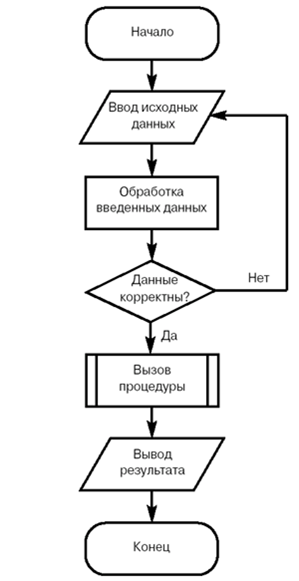
\includegraphics[width=\textwidth]{procedural}
				\end{figure}
			\end{column}

		\end{columns}

	\end{frame}

	\begin{frame}
		\frametitle{Объекты}
		
		Гради Буч:
		
		Объект "--- это мыслимая или реальная сущность, обладающая характерным поведением и отличительными характеристиками и являющаяся важной в предметной области.
		\par\bigskip
		Каждый объект имеет состояние, обладает чётко определённым поведением и уникальной идентичностью.
		\par\bigskip
		\begin{overlayarea}{\textwidth}{0.4\textheight}
				\only<1>{
					\textbf{Состояние}: в любой момент времени состояние объекта включает в себя перечень (обычно статический) свойств объекта и текущие значения (обычно динамические) этих свойств. Человек сидит и у него есть удочка.
				}
				\only<2>{
					\textbf{Поведение}: для каждого объекта существует определённый набор действий, которые с ним можно произвести. Файл в ОС можно открыть, создать и т.п.
				}
				\only<3>{
					\textbf{Уникальность}: в машинном представлении под параметром уникальности объекта чаще всего понимается адрес размещения объекта в памяти; уникальность объекта состоит в том, что всегда можно определить, указывают две ссылки на один и тот же объект или на разные объекты. Даже одинаковые монеты (абсолютно все их атрибуты одинаковы: год выпуска, номинал и т.д.), они по-прежнему остаются разными монетами.
				}
		\end{overlayarea}

	\end{frame}
	
	\begin{frame}
		\frametitle{Классы}
		
		\begin{itemize}
			\item Совокупность атрибутов и их значений характеризует объект.
			\item Все объекты одного и того же класса описываются одинаковыми наборами атрибутов.
			\item Все объекты одного и того же класса обладают одинаковым поведением.
		\end{itemize}
		\par\bigskip
		Пример 1: разные объекты класса <<Монеты>>.
		
		Пример 2: конюшня и лошадь как объекты одного класса.
		
		\begin{figure}
			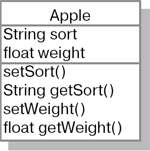
\includegraphics[width=0.2\textwidth]{class}
		\end{figure}
	\end{frame}
	
	\begin{frame}
		\frametitle{Классы}
		
		\begin{itemize}
			\item Класс имеет \textbf{имя}, которое относится ко всем объектам этого класса.
			\item В классе вводятся имена атрибутов, которые определены для объектов (атрибут=свойство=\textbf{поле}).
			\item Класс является шаблоном поведения объектов (\textbf{методы})
			\item Класс может иметь \textbf{конструктор} (constructor) "--- специальный метод, который выполняется при создании объектов.
			\item Класс может иметь \textbf{деструктор} (destructor) "--- специальный метод, который выполняется при уничтожении объектов.
		\end{itemize}
	\end{frame}	

	\begin{frame}
		\frametitle{Инкапсуляция}
		
		\textbf{Инкапсуляция} (encapsulation) "--- это сокрытие реализации класса и отделение его внутреннего представления от внешнего (интерфейса).
		\par\bigskip
		Внутри объекта данные и методы могут обладать различной степенью открытости (или доступности).
		\begin{itemize}
			\item Открытые члены класса составляют внешний интерфейс объекта "--- это та функциональность, которая доступна другим классам.
			\item Закрытыми обычно объявляются все свойства класса, а также вспомогательные методы, которые являются деталями реализации и от которых не должны зависеть другие части системы.
		\end{itemize}
		
		\textbf{Модульность} "--- благодаря сокрытию реализации за внешним интерфейсом класса можно менять внутреннюю логику отдельного класса, не меняя код остальных компонентов системы.
	\end{frame}

	\begin{frame}
		\frametitle{Наследование}
		
		\textbf{Наследование} (inheritance) "--- это отношение между классами, при котором класс использует структуру или поведение другого класса (одиночное наследование), или других (множественное наследование ) классов.
		\par\bigskip
		\begin{figure}
			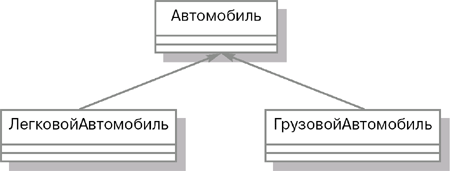
\includegraphics[width=0.5\textwidth]{inheritance}
		\end{figure}
		
		Наследование вводит иерархию <<общее/частное>>, в которой \textbf{подкласс} наследует от одного или нескольких более общих \textbf{суперклассов}.
	\end{frame}
		
	\begin{frame}
		\frametitle{Типичная задача}
		
		\underline{Пример}:
		
		Предположим, мы хотим создать векторный графический редактор, в котором нам нужно описать в виде классов набор графических примитивов "--- Point, Line, Circle, Box и т.д.
		У каждого из этих классов определим метод draw для отображения соответствующего примитива на экране.
		\par\bigskip
		\underline{Хотим}:
		
		Написать код, который при необходимости отобразить рисунок будет последовательно перебирать все примитивы, на момент отрисовки находящиеся на экране, и вызывать метод draw у каждого из них.
	\end{frame}
				
\defverbatim[colored]\lstSol{%
	\begin{lstlisting}[language=java]
Point[] p = new Point[1000];
Line[] l = new Line[1000];
Circle[] c = new Circle[1000];
Box[] b = new Box[1000];
//...
//...
for(int i = 0; i < p.length;i++) {
	if(p[i]!=null) p[i].draw();
}
for(int i = 0; i < l.length;i++) {
	if(l[i]!=null) l[i].draw();
}
for(int i = 0; i < c.length;i++) {
	if(c[i]!=null) c[i].draw();
}
for(int i = 0; i < b.length;i++) {
	f(b[i]!=null) b[i].draw();
}
	\end{lstlisting}
}				
	\begin{frame}
		\frametitle{Решение 1}
		
		\lstSol
	\end{frame}

\defverbatim[colored]\lstSolB{%
	\begin{lstlisting}[language=java]
Point p[] = new Point[1000];
p[0] = new Circle();
p[1] = new Point();
p[2] = new Box();
p[3] = new Line();
//...
for(int i = 0; i < p.length;i++) {
	if(p[i]!=null) p[i].draw();
}
	\end{lstlisting}
}				
	\begin{frame}
		\frametitle{Решение 2}
		
		\begin{figure}
			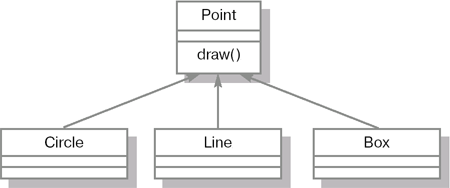
\includegraphics[width=0.5\textwidth]{solution2}
		\end{figure}
		
		\lstSolB
	\end{frame}		

\defverbatim[colored]\lstPoly{%
	\begin{lstlisting}[language=java]
void println(); 
void println(boolean x);
void println(String x);
	\end{lstlisting}
}
	\begin{frame}
		\frametitle{Полиморфизм}

		\textbf{Полиморфизм} (polymorphism) "--- положение теории типов, согласно которому имена (например, переменных) могут обозначать объекты разных (но имеющих общего родителя) классов.
		\par\bigskip
		Процедурный полиморфизм предполагает возможность создания нескольких процедур или функций с одним и тем же именем, но разным количеством или различными типами передаваемых параметров "--- \textbf{перегрузка} (overloading) функций.
		\lstPoly
	\end{frame}
			
\defverbatim[colored]\lstConsoleRead{%
	\begin{lstlisting}[language=java]
	import java.util.Scanner;
	
	public class InputExp {
		public static void main(String[] args) {
			String name;
			int age;
			Scanner in = new Scanner(System.in);

			name = in.nextLine();
			age = in.nextInt();
			in.close();

			System.out.println("Name :" + name);
			System.out.println("Age :" + age);
		}
	}
	\end{lstlisting}
}
\begin{frame}
	\frametitle{Чтение с консоли}

	\lstConsoleRead
\end{frame}

\defverbatim[colored]\lstFileRead{%
	\begin{lstlisting}[language=java]
import java.io.FileInputStream;
import java.io.FileNotFoundException;
import java.util.Scanner;
public class ScannerReadFile {
	public static void main(String[] args) {
		try {
			FileInputStream fileStream = new FileInputStream("test.txt");

			Scanner scanner = new Scanner(fileStream);
			while (scanner.hasNextLine()) {
				String line = scanner.nextLine();
				System.out.println(line);
			}
		} catch (FileNotFoundException e) {
			System.out.println("File not found");
		}
	}
}
	\end{lstlisting}
}
\begin{frame}
	\frametitle{Чтение из файла}
	
	\lstFileRead
\end{frame}

	\section{Семинар 3}
	\subsection{Курсовой проект}
	
	\begin{frame}
		\frametitle{Темы проектов}
		
		\begin{itemize}
			\item Научные:
			\begin{itemize}
				\item распознавание образов с помощью нейросетей,
				\item машинное обучение,
				\item мультиагентные системы.
			\end{itemize}
			\item Учебные:
			\begin{itemize}
				\item Микро-фотошоп "--- набор различных фильтров для обработки изображений,
				\item Редактор формул "--- набор формул, их сохранение и конвертация в \LaTeX и MathType,
				\item Реактор "--- моделирование работы гомогенного ураново-графитого ядерного реактора,
				\item Столкновение тел "--- помолекулярное моделирование столкновения малых тел с учётом различных взаимодействий,
				\item Графы и сети "--- программа для работы с сетями а алгоритмами на них (коммивояжёр, клика и т.~п.),
			\end{itemize}
		\end{itemize}
	\end{frame}

	\begin{frame}
		\frametitle{Темы проектов}
		
		\begin{itemize}
			\item Учебные:
			\begin{itemize}
				\item Дорожное движение "--- моделирование дорожного движения в городе с некоторой картой,
				\item Фракталы "--- построение множеств Жюлиа для различных отображений, исследование критических точек,
			\end{itemize}
			\item Развлекательные:
			\begin{itemize}
				\item Экология "--- двумерная трёхкомпонентная экологическая модель,
				\item Жизнь "--- генетический варианта игры жизнь, обобщение клеточных автоматов,
				\item Чат "--- программа обмена пользовательскими сообщениями (Android, desktop),
				\item Танчики "--- многопользовательская игра с ботами и web-интерфейсом.
			\end{itemize}
		\end{itemize}
	\end{frame}					

	\begin{frame}
		\frametitle{Требования к проекту. Общие}
		
		\begin{itemize}
			\item Разработка в команде из 3--4 человек.
			\item Использование системы контроля версий (Git, SVN).
			\item Презентация выбранного проекта с четкой формулировкой будущих работ каждого участника и сроков.
			\item Согласование архитектуры проекта.
			\item Каждый участник должен соблюсти все технические требования в своём коде.
			\item Проект должен быть доведен до планируемого рабочего состояния.
			\item Презентация по итогам завершения проекта "--- что получилось, что нет.
		\end{itemize}
	\end{frame}

	\begin{frame}
		\frametitle{Требования к проекту. Технические}
		
		\begin{itemize}
			\item Обработка ошибок как внутренних, так и ошибок непредвиденного использования.
			\item Применение многопоточного программирования, как минимум на уровне отделения рабочих процессов от интерфейса пользователя.
			\item Использование стандартных классов для работы с коллекциями.
			\item Комментарии в тексте программы (JavaDoc, \_\_doc\_\_): в начале каждого класса, для каждой публичной функции и поля.
			\item Оформление кода: соблюдение CodeStyle для данного языка программирования (отступы, правильное название полей и методов и т.~д.).
			\item Наличие файлов сборки (Ant, Maven, make).
		\end{itemize}
	\end{frame}

	\begin{frame}
		\frametitle{Допуск к проекту: задачи}
		
		\begin{itemize}
			\item Обе задачи должны быть выполнены на выбранном командой языке программирования.
			\item Для обоих задач должен быть дополнительный тестовый класс, в котором демонстрируется функциональность реализованной коллекции или алгоритма.
			\item Должны быть соблюдены CodeStyle и присутствовать комментарии.
			\item Задача \No1: нельзя использовать стандартные классы коллекций, только массивы.
			\item Задача \No2: выбор места для распараллеливания алгоритма "--- часть решения задачи.
		\end{itemize}
	\end{frame}

\defverbatim[colored]\lstAgregation{%
	\begin{lstlisting}[language=java]
public class Fish {
	private Aquarium home;
	public Fish() {
	}
}

public class Aquarium {
	private Fish inhabitants[];
	public Aquarium() {
	}
}
	\end{lstlisting}
}
	\subsection{Связи между классами}
	\begin{frame}
		\frametitle{Агрегация}
		
		\begin{figure}
			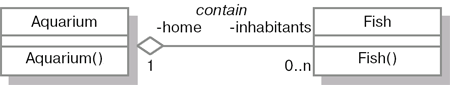
\includegraphics[width=0.7\textwidth]{agregation}
		\end{figure}
		\lstAgregation
	\end{frame}

\defverbatim[colored]\lstAssociation{%
	\begin{lstlisting}[language=java]
public class Programmer {
	private Computer computers[];
	public Programmer() {
	}
}

public class Computer {
	private Programmer programmers[];
	public Computer() {
	}
}
	\end{lstlisting}
}
	\begin{frame}
		\frametitle{Ассоциация}
		
		\begin{figure}
			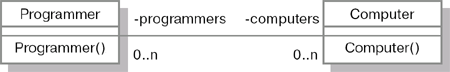
\includegraphics[width=0.7\textwidth]{association}
		\end{figure}
		\lstAssociation
	\end{frame}	

\defverbatim[colored]\lstObject{%
	\begin{lstlisting}[language=java]
Point p7=new Point(2,3);
Point p8=new Point(2,3);
System.out.println(p1.equals(p2));

System.out.println(p7.hashCode() == p8.hashCode());
System.out.println(p7.toString());

Point@92d351
	\end{lstlisting}
}
	\subsection{Стандартные классы}
	\begin{frame}
		\frametitle{Класс Object}
		Каждый класс в Java неявно наследуется от класса Object. В нем определены некоторые методы, которые, таким образом, есть у любого класса.
		\begin{itemize}
			\item \textbf{equals()} "--- служит для сравнения объектов по значению, а не по ссылке.
			\item \textbf{hashCode()} "--- представить любой объект целым числом.
			\item \textbf{toString()} "--- позволяет получить текстовое описание любого объекта.
		\end{itemize}
		\lstObject
	\end{frame}

\defverbatim[colored]\lstString{%
	\begin{lstlisting}[language=java]
String s1 = "abc";
String s2 = "abc";
String s3 = "a"+"bc";

System.out.println(s1==s2);
System.out.println(s1==s3);
System.out.println(s1.equals(s2));
	\end{lstlisting}
}

	\begin{frame}
		\frametitle{Класс String}
		
		Класс String занимает в Java особое положение:
		
		\begin{itemize}
			\item экземпляры только этого класса можно создавать без использования ключевого слова \textbf{new},
			\item каждый строковый литерал порождает экземпляр String, и это единственный литерал (кроме null), имеющий объектный тип,
			\item много полезных методов: \textbf{length()}, \textbf{split(String regex)}, \textbf{substring(int beginIndex, int endIndex)}, \textbf{toCharArray()}, \textbf{charAt(int index)} и др.
		\end{itemize}
		\lstString
	\end{frame}

	\begin{frame}
		\frametitle{Java из командной строки}
		
		\begin{itemize}
			\item javac HelloWorld.java
			\item java -classpath . HelloWorld
		\end{itemize}
		
		Отделяем исходники (папка src) и бинарные файлы (папка bin).
		\begin{itemize}
			\item javac -d bin HelloWorld.java
			\item java -classpath ./bin HelloWorld
		\end{itemize}
		
		Помещаем исходный класс в пакет ru.mipt.cs.
		\begin{itemize}
			\item javac -d bin ru/mipt/cs/helloworld/HelloWorld.java
			\item java -classpath ./bin ru.mipt.cs.helloworld.HelloWorld
		\end{itemize}				
		
		Несколько файлов в проекте.		
		\begin{itemize}
			\item javac -d ../bin ru/mipt/cs/helloworld/HelloWorld.java
			\item java -classpath ./bin ru.mipt.cs.helloworld.HelloWorld
		\end{itemize}				
	\end{frame}

	\section{Семинар 4}
	\subsection{Имена и области видимости}
	\begin{frame}
		\frametitle{Пакеты}
		
		\begin{itemize}
			\item Пакеты (packages) в Java "--- это способ логически группировать классы.
			\item В файловой системе они представлены директориями.
			\item Аналогично директории, пакет может внутри кроме классов содержать и другие пакеты "--- свои элементы.
			\item Примеры: java.lang, com.sun.misc, ru.mipt.dgap.cs025.project.
		\end{itemize}
	\end{frame}
	
	\begin{frame}
		\frametitle{Простые и составные имена}
		
		\begin{itemize}
			\item Простое имя классов, полей и методов дается при объявлении: Object, String, Point, toString(), PI, InnerClass.
			\item Чтобы получить составное имя, надо к имени родителя, в котором находится элемент, через точку добавить простое имя элемента:
			
			java.lang.Object, 
			
			java.lang.reflect.Method, 
			
			com.myfirm.MainClass, 
			
			ref.toString(), 
			
			java.lang.Math.PI, 
			
			OuterClass.InnerClass
		\end{itemize}
	\end{frame}

\defverbatim[colored]\lstScope{%
	\begin{lstlisting}[language=java]
class Pointer {
	int x, y;

	int getX() {
		return x; // simple name
	}
}

class Test {
	void main() {
		Pointer p = new Pointer();
		p.x = 3; // complex name
	}
}
	\end{lstlisting}
}

	\begin{frame}
		\frametitle{Область видимости}
		
		У каждого имени есть область видимости (scope).
		
		\lstScope
	\end{frame}

	\begin{frame}
		\frametitle{Classpath}
		
		\begin{itemize}
			\item Не всегда удобно хранить все файлы в одном каталоге
			\item Удобно распространять классы в виде JAR (Java ARchive) или ZIP архивов, для ускорения загрузки через сеть.
			\item Существует специальная переменная окружения classpath (по аналогии с path) "--- её значение должно состоять из путей к каталогам или архивам, разделённых точкой с запятой
			
			.;C:/java/classes;D:/lib/3Dengine.zip;D:/lib/fire.jar
		\end{itemize}
	\end{frame}


	\begin{frame}
		\frametitle{Модуль компиляции}
		
		\begin{itemize}
			\item Модуль компиляции (compilation unit) хранится в текстовом .java-файле и является единичной порцией входных данных для компилятора. Он состоит из трёх частей:
			\begin{itemize}
				\item объявление пакета;
				\item import-выражения;
				\item объявления верхнего уровня.
			\end{itemize}
			\item Порядок работы import:
			\begin{itemize}
				\item сначала просматриваются выражения, импортирующие типы;
				\item затем другие типы, объявленные в текущем пакете, в том числе в текущем модуле компиляции;
				\item наконец, просматриваются выражения, импортирующие пакеты.
			\end{itemize}
			\item Область видимости объявления верхнего уровня по умолчанию "--- пакет.
		\end{itemize}
	\end{frame}

	\begin{frame}
		\frametitle{Области видимости}
		
		\begin{itemize}
			\item Область видимости доступного пакета "--- вся программа.
			\item Областью видимости импортированного типа являются все объявления верхнего уровня в этом модуле компиляции.
			\item Областью видимости класса верхнего уровня является пакет, в котором он объявлен.
			\item Область видимости элементов классов "--- это все тело типа, в котором они объявлены, доступ через имя класса или зарезервированные слова \textbf{this} и \textbf{super}.
			\item Аргументы метода, конструктора или обработчика ошибок видны только внутри этих конструкций и не могут быть доступны извне.
			\item Область видимости локальных переменных начинается с момента их инициализации и до конца блока, в котором они объявлены.
		\end{itemize}
	\end{frame}

\defverbatim[colored]\lstShad{%
	\begin{lstlisting}[language=java]
class Human {
	int age;
	void setAge(int age) {
		this.age = age; // OK
	}
}
	\end{lstlisting}
}
\defverbatim[colored]\lstObscur{%
	\begin{lstlisting}[language=java]
public class Obscuring {
	static Point Test = new Point(3, 2);
	public static void main(String s[]) {
		System.out.print(Test.x);
	}
}

class Test {
	static int x = -5;
}
	\end{lstlisting}
}
	\begin{frame}
		\frametitle{Перекрытие областей видимости}
		
		\begin{overlayarea}{\textwidth}{0.5\textheight}
			\begin{itemize}
				\only<1>{
					\item Затеняющее объявление (shadowing)
					\lstShad
				}
				\only<2>{
					\item Заслоняющее объявление (obscuring)
					\lstObscur
				}
			\end{itemize}
		\end{overlayarea}

	\end{frame}

	\begin{frame}
		\frametitle{Соглашения по именованию}
		
		\begin{itemize}
			\item Имя каждого пакета начинается с маленькой буквы и представляет собой, как правило, одно недлинное слово, возможно с подчеркиванием (com.sun.image.codec.jpeg, org.omg.CORBA.ORBPackage, oracle.jdbc.driver).
			\item Имена типов начинаются с большой буквы и могут состоять из нескольких слов, каждое следующее слово также начинается с большой буквы (Human, HighGreenOak, ArrayIndexOutOfBoundsException, Runnable, Serializable, Cloneable).
			\item Имена методов должны быть глаголами и обозначать действия, которые совершает данный метод. Имя должно начинаться с маленькой буквы, но может состоять из нескольких слов, причём каждое следующее слово начинается с заглавной буквы.
		\end{itemize}
	\end{frame}
	
	\begin{frame}
		\frametitle{Соглашения по именованию}
		
		\begin{itemize}
			\item Поля класса имеют имена, записываемые в том же стиле, что и для методов, начинаются с маленькой буквы, могут состоять из нескольких слов, каждое следующее слово начинается с заглавной буквы. Имена должны быть существительными, например, поле name в классе Human, или size в классе Planet.
			\item Имена констант состоят из последовательности слов, сокращений, аббревиатур. Записываются они только большими буквами, слова разделяются знаками подчеркивания (PI, MIN\_VALUE, MAX\_VALUE, COLOR\_RED, COLOR\_GREEN, COLOR\_BLUE).
			\item Имена локальных переменных, параметров методов и обработчиков ошибок, как правило, довольно короткие, но, тем не менее, должны быть осмыслены. Например, можно использовать аббревиатуру (имя cp для ссылки на экземпляр класса ColorPoint) или сокращение (buf для buffer).
		\end{itemize}
	\end{frame}

	\begin{frame}
		\frametitle{CVS "--- Control Version Systems}
		Система контроля версий "--- комплекс программного обспечения для обеспечения коллективной работы с исходным кодом, а так же отслеживания изменений в нем.
		
		Типичные задачи, которые позволяет решить система контроля версий:
		
		\begin{itemize}
			\item Узнать, что я поменял с момента последней <<живой>> копии?
			\item Получить исходник установленной месяц назад системы.
			\item Параллельная работа 2-х и более человек над одним исходником.
		\end{itemize}
		
		Выбираем из двух систем контроля версий:
		\begin{itemize}
			\item Subversion.
			\item GIT/GitHub.
		\end{itemize}
	\end{frame}

	\subsection{Модификаторы доступа}
\defverbatim[colored]\lstPubHum{%
	\begin{lstlisting}[language=java]
public class Human {
	public int age;
}

Human h = new Human(); 
int i=h.age;
	\end{lstlisting}
}	
\defverbatim[colored]\lstPrivHum{%
	\begin{lstlisting}[language=java]
public class Human {
	private int age;

	public int getAge() {
		return age;
	}

	public void setAge(int a) {
		age=a;
	}
}

Human h = new Human();
int i=h.getAge();
	\end{lstlisting}
}	
	\begin{frame}
		\frametitle{Сокрытие реализации}
		
		Модификаторы доступа вводятся для защиты, или избавления, пользователя от излишних зависимостей от деталей внутренней реализации.
		\begin{overlayarea}{\textwidth}{0.7\textheight}
			\only<1>{
				\lstPubHum	
			}
			\only<2>{
				\lstPrivHum
			}
		\end{overlayarea}
	\end{frame}

\defverbatim[colored]\lstChangeHum{%
	\begin{lstlisting}[language=java]
public class Human {
	private/* int */double age;

	public int getAge() {
		return (int) Math.round(age);
	}
	public void setAge(int a) {
		age = a;
	}

	public double getExactAge() {
		return age;
	}
	public void setExactAge(double a) {
		age = a;
	}
}
	\end{lstlisting}
}	
	\begin{frame}
		\frametitle{Изменение реализации}
		
		\lstChangeHum
	\end{frame}
	
	\begin{frame}
		\frametitle{Уровни доступа}
		
		В Java модификаторы доступа указываются для:
		\begin{itemize}
			\item классов объявления верхнего уровня,
			\item элементов класса (полей, методов, внутренних типов),
			\item конструкторов классов.
		\end{itemize}
		
		Все четыре уровня доступа имеют только элементы типов и конструкторы. Это:
		\begin{itemize}
			\item public,
			\item private,
			\item protected,
			\item если не указан ни один из этих трёх типов, то уровень доступа определяется по умолчанию (default).
		\end{itemize}
	\end{frame}

\defverbatim[colored]\lstClassSchema{%
	\begin{lstlisting}[language=java, basicstyle=\tiny]
[public] [final] class ValidClassName [extends ParentClassName] {
	[public,private,protected] [static] [final] int valName [=0];
	[public,private,protected] [static] [final] MyType valName2 [=null];
	
	[public,private,protected] ValidClassName([int paramName][, [final] MyType paramName2][...]) [throws ExceptionName]{
		[super(...);]...
	}

	[public,private,protected] [static] [final] [void, int, MyType] methodName([int paramName][, [final] MyType paramName2][...]) [throws ExceptionName]{
		[super. methodName(...);]...
	}
}
	\end{lstlisting}
}

	\begin{frame}
		\frametitle{Шаблон объявления класса}
		
		\lstClassSchema
	\end{frame}

	\section{Семинар 5}
	\subsection{Объектная модель}
	\begin{frame}
		\frametitle{Контекст выполнения}
		
		К статическому контексту выполнения относятся:
		\begin{itemize}
			\item статические методы,
			\item статические поля.
		\end{itemize}

		Остальные части кода относятся к динамическому контексту:		
		\begin{itemize}
			\item обычные методы,
			\item обычные поля,
			\item конструкторы.
		\end{itemize}
	\end{frame}

\defverbatim[colored]\lstStat{%
	\begin{lstlisting}[language=java]
class Test {
	public void process() {
	}
	
	public static void main(String s[]) {
		// process(); - error!

		Test test = new Test();
		test.process(); // OK!
	}
}
	\end{lstlisting}
}
	\begin{frame}
		\frametitle{Статический контекст}
		
		\lstStat
	\end{frame}

\defverbatim[colored]\lstAbstract{%
	\begin{lstlisting}[language=java]
// Base operation
public abstract class Operation {
	public int calculate(int a, int b){}
}

class Addition extends Operation {
	public int calculate(int a, int b) {
		return a+b;
	}
}

class Subtraction extends Operation {
	public int calculate(int a, int b) {
		return a-b;
	}
}
	\end{lstlisting}
}
	\begin{frame}
		\frametitle{Абстрактные классы}
		
		\lstAbstract
	\end{frame}

\defverbatim[colored]\lstAbstractMeth{%
	\begin{lstlisting}[language=java]
	// Base operation
	public abstract class Operation {
		public abstract int calculate(int a, int b);
	}
	
	class Addition extends Operation {
		public int calculate(int a, int b) {
			return a+b;
		}
	}
	
	class Subtraction extends Operation {
		public int calculate(int a, int b) {
			return a-b;
		}
	}
	\end{lstlisting}
}
	\begin{frame}
		\frametitle{Абстрактный метод}
		
		\lstAbstractMeth
	\end{frame}

\defverbatim[colored]\lstAbsExample{%
	\begin{lstlisting}[language=java]
class Test {
	public static void main(String s[]) {
		Operation o1 = new Addition();
		Operation o2 = new Subtraction();
		
		o1.calculate(2, 3);
		o2.calculate(3, 5);
	}
}
	\end{lstlisting}
}
	\begin{frame}
		\frametitle{Пример использования абстрактного класса}
		
		\lstAbsExample
	\end{frame}

\defverbatim[colored]\lstInterface{%
	\begin{lstlisting}[language=java]
public interface Drawable extends Colorable, Resizable {
	public final static int RIGHT = 1;
	int LEFT = 2;
	int UP = 3;
	int DOWN = 4;

	public abstract void moveRight();
	void moveLeft();
	void moveUp();
	void moveDown();
}
	\end{lstlisting}
}
	\begin{frame}
		\frametitle{Интерфейс}
		
		\lstInterface
	\end{frame}

\defverbatim[colored]\lstInterExample{%
	\begin{lstlisting}[language=java]
public interface InsectConsumer {
	void consumeInsect(Insect i);
}
// Rosianka
class Sundew extends Plant implements InsectConsumer {
	public void consumeInsect(Insect i) {
		// ...
	}
}
// Lastochka
class Swallow extends Bird implements InsectConsumer {
	public void consumeInsect(Insect i) {
		// ...
	}
}
	\end{lstlisting}
}
	\begin{frame}
		\frametitle{Использование интерфейсов}
		
		\lstInterExample
	\end{frame}

\defverbatim[colored]\lstInterExContinue{%
	\begin{lstlisting}[language=java]
// Muravied
class AntEater extends Mammal implements InsectConsumer {
	public void consumeInsect(Insect i) {
		// ...
	}
}

class FeedWorker extends Worker {
	public void feedOnInsects(InsectConsumer consumer) {
		consumer.consumeInsect(new Insect());
	}
}
	\end{lstlisting}
}
	\begin{frame}
		\frametitle{Использование интерфейсов}
		
		\lstInterExContinue
	\end{frame}		
	
	\subsection{Преобразование типов}
\defverbatim[colored]\lstTypeCasting{%
	\begin{lstlisting}[language=java]
long a = 3;
a = 5 + 'A' + a;
print("a=" + Math.round(a / 2F));
int b=1;
byte c=(byte)-b;
int i=c;
	\end{lstlisting}
}	
	\begin{frame}
		\frametitle{Автоматическое преобразование}
		
		Тип устанавливается на основе структуры применяемых выражений и типов литералов, переменных и методов, используемых в этих выражениях.
		
		\lstTypeCasting
	\end{frame}

\defverbatim[colored]\lstCastingPrim{%
	\begin{lstlisting}[language=java]
long d=111111111111L;
float f = d;
a = (long) f;
print(d);

print((byte)383); 
print((byte)384); 
print((byte)-384);
char ch=40000; 
print((short)ch);
	\end{lstlisting}
}
	\begin{frame}
		\frametitle{Примитивные типы}
		
		\begin{itemize}
			\item \textbf{Расширение примитивного типа} (widening primitive) "--- автоматическое.
			\item \textbf{сужение примитивного типа} (narrowing primitive) "--- явно, т.~к. можно потерять данные.
		\end{itemize}
		\lstCastingPrim
	\end{frame}
	
\defverbatim[colored]\lstCastingObjEx{%
	\begin{lstlisting}[language=java]
class Parent {
	int x;
}

class Child extends Parent {
	int y;
}

class Child2 extends Parent {
	int z;
}
	\end{lstlisting}
}	
	\begin{frame}
		\frametitle{Объектные типы. Пример}
		
		\lstCastingObjEx
	\end{frame}			

\defverbatim[colored]\lstCastingObj{%
	\begin{lstlisting}[language=java]
Parent p1=new Child();
Parent p2=new Child2();
Parent p3=null;

Parent p = new Child();
Child c = (Child) p; // OK!
Parent p2 = new Child2();
Child c2 = (Child) p2; // Error!
if (p2 instanceof Child) {
	Child c3 = (Child) p2;
}
	\end{lstlisting}
}	
	\begin{frame}
		\frametitle{Преобразование объектных типов}
		
		\begin{itemize}
			\item \textbf{Расширение объектного типа} (widening reference) "--- автоматическое.
			\item \textbf{Сужение объектного типа} (narrowing reference) "--- явно, т.~к. может быть ClassCastException.
		\end{itemize}
		
		\lstCastingObj
	\end{frame}

	\begin{frame}
	\frametitle{Оставшиеся случаи}
	
		\begin{itemize}
			\item \textbf{Преобразование к строке} (String) "--- автоматически любые типы.
			\item \textbf{Запрещенные преобразования} (forbidden):
			\begin{itemize}
				\item переходы от любого ссылочного типа к примитивному, от примитивного "--- к ссылочному (кроме преобразований к строке);
				\item тип boolean нельзя привести ни к какому другому типу, кроме boolean (за исключением приведения к строке);
				\item невозможно привести друг к другу типы, находящиеся не на одной, а на соседних ветвях дерева наследования и др.
			\end{itemize}
		\end{itemize}
	\end{frame}	
	
	\subsection{Исключительные ситуации}
	\begin{frame}
		\frametitle{Исключительные ситуации}
		
		Ошибки могут возникать как по причине недостаточной внимательности программиста (отсутствует нужный класс, или индекс массива вышел за допустимые границы), так и по независящим от него причинам (произошел разрыв сетевого соединения, сбой аппаратного обеспечения, например, жесткого диска и др.).
		
		\par\bigskip
		При возникновении исключительной ситуации управление передается от кода, вызвавшего исключительную ситуацию, на ближайший блок \textbf{catch} (или вверх по стеку) и создается объект, унаследованный от класса \textbf{Throwable}, или его потомков, который содержит информацию об исключительной ситуации и используется при ее обработке.
	\end{frame}

\defverbatim[colored]\lstExceptions{%
	\begin{lstlisting}[language=java]
try {
	if (p.x == 0) {
		throw new SomeExceptionClass();
	} else {
		throw new AnotherExceptionClass();
	}
	// ...
} catch (SomeExceptionClass e) { // from common to special types
	// ...
} catch (AnotherExceptionClass e) {
	// ...
} finally {
}
	\end{lstlisting}
}
	\begin{frame}
		\frametitle{Обработка исключений}
		
		\lstExceptions
	\end{frame}

	\begin{frame}
		\frametitle{Проверяемые и непроверяемые исключения}
		
		\begin{figure}
			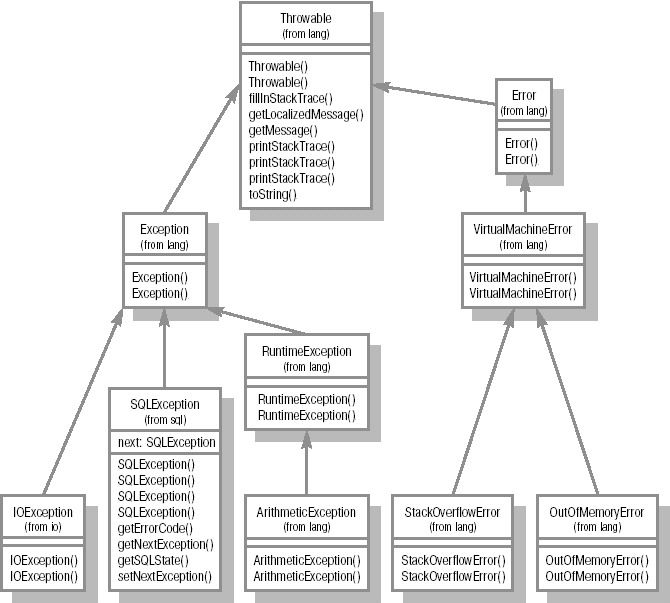
\includegraphics[width=0.7\textwidth]{exceptions.png}
		\end{figure}
	\end{frame}

	\section{Семинар 6}
	\subsection{Потоки}
	\begin{frame}
		\frametitle{Зачем нужно организовывать потоки}
		
		\begin{itemize}
			\item Выполнение задач, где действительно требуется выполнять несколько действий одновременно: сервер общего пользования, активные игры (опрашивание клавиатуры и других устройства ввода) и т.д.
			\item Вычислительное устройство "--- лишь один из ресурсов, необходимых для выполнения задач. Всегда есть оперативная память, дисковая подсистема, сетевые подключения, периферия и т.~д., которые необходимо делить. Пример: пользователю требуется распечатать большой документ и скачать большой файл из сети.
			\item Более гибко управлять выполнением задач: реализация кнопки Cancel, регулирование приоритетами и т.~п.
			\item Обслуживающие потоки: автоматический сборщик мусора в Java запускается в виде фонового (низкоприоритетного) процесса "--- демон (daemon).
		\end{itemize}
	\end{frame}

\defverbatim[colored]\lstThread{%
	\begin{lstlisting}[language=java]
public class MyThread extends Thread {
	public void run() {
		// long calculation
		long sum = 0;
		for (int i = 0; i < 1000; i++) {
			sum += i;
		}
		System.out.println(sum);
	}
}

MyThread t = new MyThread();
t.start();
	\end{lstlisting}
}
	\begin{frame}
		\frametitle{Создание Thread}
		
		\lstThread
	\end{frame}

\defverbatim[colored]\lstRunnable{%
	\begin{lstlisting}[language=java]
public class MyRunnable implements Runnable {
	public void run() {
		// long calculation
		long sum = 0;
		for (int i = 0; i < 1000; i++) {
			sum += i;
		}
		System.out.println(sum);
	}
}

Runnable r = new MyRunnable();
Thread t = new Thread(r);
t.start();
	\end{lstlisting}
}
	\begin{frame}
		\frametitle{Создание Runnable}
		
		\lstRunnable
	\end{frame}

\defverbatim[colored]\lstTestRunnable{%
	\begin{lstlisting}[language=java, basicstyle=\tiny]
public class ThreadTest implements Runnable {
	public void run() {
		double calc;
		for (int i = 0; i < 50000; i++) {
			calc = Math.sin(i * i);
			if (i % 10000 == 0) {
				System.out.println(getName() + " counts " + i / 10000);
			}
		}
	}

	public String getName() {
		return Thread.currentThread().getName();
	}
	
	public static void main(String s[]) {
		Thread t[] = new Thread[3];
		for (int i = 0; i < t.length; i++) {
			t[i] = new Thread(new ThreadTest(), "Thread " + i);
		}
	
		for (int i = 0; i < t.length; i++) {
			t[i].start();
			System.out.println(t[i].getName() + " started");
		}
	}
}
	\end{lstlisting}
}
	\begin{frame}
		\frametitle{Именованные потоки}
		
		\lstTestRunnable
	\end{frame}

\defverbatim[colored]\lstPriority{%
	\begin{lstlisting}[language=java]
public static void main(String s[]) {
	Thread t[] = new Thread[3];
	for (int i = 0; i < t.length; i++) {
		t[i] = new Thread(new ThreadTest(), "Thread " + i);
		t[i].setPriority(Thread.MIN_PRIORITY + (Thread.MAX_PRIORITY - Thread.MIN_PRIORITY) / t.length* i);
	}

	for (int i = 0; i < t.length; i++) {
		t[i].start();
		System.out.println(t[i].getName() + " started");
	}
}
	\end{lstlisting}
}
	\begin{frame}
		\frametitle{Приоритеты}
		
		\lstPriority
	\end{frame}

\defverbatim[colored]\lstDemonSt{%
	\begin{lstlisting}[language=java]
class ThreadTest implements Runnable {

	public final static ThreadGroup GROUP = new ThreadGroup("Daemon demo");
	private int start;
	
	public ThreadTest(int s) {
		start = (s % 2 == 0) ? s : s + 1;
		new Thread(GROUP, this, "Thread " + start).start();
	}

	public static void main(String s[]) {
		new ThreadTest(16);
		new DaemonDemo();
	}
	\end{lstlisting}
}

\defverbatim[colored]\lstDemonEnd{%
	\begin{lstlisting}[language=java]
	public void run() {
		for (int i = start; i > 0; i--) {
			try {
				Thread.sleep(300);
			} catch (InterruptedException e) {
			}
		
			if (start > 2 && i == start / 2) {
				new ThreadTest(i);
			}
		}
	}
}
	\end{lstlisting}
}

\defverbatim[colored]\lstDemonClass{%
	\begin{lstlisting}[language=java]
class DaemonDemo extends Thread {
	public DaemonDemo() {
		super("Daemon demo thread");
		setDaemon(true);
		start();
	}

	public void run() {
		Thread threads[] = new Thread[10];
		while (true) {
	\end{lstlisting}
}

\defverbatim[colored]\lstDemonWhile{%
	\begin{lstlisting}[language=java]
			int count = ThreadTest.GROUP.activeCount();
				if (threads.length < count)
					threads = new Thread[count + 10];
					count = ThreadTest.GROUP.enumerate(threads);

					for (int i = 0; i < count; i++) {
						System.out.print(threads[i].getName() + ", ");
					}
					System.out.println();
					
					try {
						Thread.sleep(300);
					} catch (InterruptedException e) {}
		}
	}
}
	\end{lstlisting}
}
	\begin{frame}
		\frametitle{Поток"--~демон}
		
		\begin{overlayarea}{\textwidth}{\textheight}
			\only<1>{
				\lstDemonSt
			}
			\only<2>{
				\lstDemonEnd
			}
			\only<3>{
				\lstDemonClass
			}
			\only<4>{
				\lstDemonWhile
			}
		\end{overlayarea}
	\end{frame}

	%	\begin{frame}
	%		\frametitle{Цели курса}
	%		
	%		\begin{itemize}
	%			\item
	%		\end{itemize}
	%	\end{frame}
	
\end{document}
	
	
